\documentclass[
  lualatex,
  aspectratio=169,
  fleqn,
  14pt,
]{beamer}
\batchmode

\usetheme[progressbar=frametitle]{Metropolis}
%\setbeameroption{show notes on second screen=bottom}

\usepackage{xparse}
\usepackage{mathtools,amssymb}
\usepackage{graphicx,xcolor}
\usepackage{pxrubrica}
\usepackage{calc}
\usepackage[absolute,overlay]{textpos}
%\usepackage{enumitem}
\usepackage[1.7]{bxpdfver}
\usepackage{pdfcomment}
\usepackage{ulem}
\usepackage{stackengine}
\usepackage{appendixnumberbeamer}
\usepackage{tabto}
\usepackage[superscript]{cite}
\usepackage{siunitx}

\RenewDocumentCommand\citeform{m}{[#1]}

% フォント
\usepackage[lining,tabular,sfdefault]{FiraSans}
\usepackage[mathrm=sym,mathbf=sym]{unicode-math}
\setmathfont{Fira Math}
\usepackage[no-math,deluxe,haranoaji]{luatexja-preset}
\RenewDocumentCommand\kanjifamilydefault{}{\gtdefault}

% 打ち消し線関連
\RenewDocumentCommand\ULthickness{}{.1\zh}
% 二重打ち消し
\NewDocumentCommand\dsout{m}{%
  \stackengine{.2\zh}{#1}{%
    \stackengine{-.3\zh}{\sout{\hphantom{#1}}}{\sout{\hphantom{#1}}}{O}{c}{F}{F}{L}%
  }{O}{c}{F}{F}{L}}

% 下に文字置くやつ
\NewDocumentCommand\replace{mm}{%
  \smash{\stackengine{-1\zh}{\dsout{#1}}{#2}{O}{c}{F}{F}{L}}}

% 床関数
\DeclarePairedDelimiter\floor\lfloor\rfloor

\usepackage{hyperref}

\title{郵便を用いた超低速IP通信システムの検討}
\subject{エンジニア作業飲み集会\#147}
\author{%
  \texorpdfstring{%
    \ltjsetparameter{autospacing=false, autoxspacing=false}
    上羽 未栞\inst{\dag}\inst{a)}\and
    信濃 眞伊\inst{\dag}\inst{b)}\and
    佐伯 真紘\inst{\dag}\inst{c)}\and
    一式 すみれ\inst{\dag}\inst{d)}}
    {上羽 未栞\and 信濃 眞伊\and 佐伯 真紘\and 一式 すみれ}}
\institute{
  \tabcolsep = .25\zw
  \begin{tabular}{rl}
    \inst{\dag} & 東京広域電話網, \url{https://tkytel.github.io/}\\
    a) & a.k.a. KusaReMKN, \url{mkn@kusaremkn.com}\\
    b) & \url{me@shinanomai.xyz}\\
    c) & a.k.a. Nejikugi, \url{me@scrwnl.eu.org}\\
    d) & a.k.a. yude, \url{i@yude.jp}
  \end{tabular}
}
\keywords{LoLLIPoP; 郵便; TCP/IP; RFC 1149}
\date{2025-11-07}

\begin{document}

\begin{frame}
  \titlepage
  \thispagestyle{empty}
  \note{
    はじまるよ〜。

    郵便を用いた超低速IP通信システムの検討と題して、
    東京広域電話網のLoLLIPoPチームを代表して
    上羽未栞が発表するよ。
  }
\end{frame}

\begin{frame}
  \frametitle{今回のおはなし}

  \vspace{.25\zh}
  \tableofcontents
  \note{
    今回の発表の流れはこんな感じだよ。
    おおよそ25分くらいで進められたらいいな。
  }
\end{frame}

\begin{frame}
  \frametitle{今回の発表に関係するひとびと}

  \begin{center}
    \tabcolsep = .25\zw
    \begin{tabular}{cccc}
      \includegraphics[width=0.20\linewidth]{./images/mikan.png} &
      \includegraphics[width=0.20\linewidth]{./images/shinanomai.jpg} &
      \includegraphics[width=0.20\linewidth]{./images/nejikugi.jpg} &
      \includegraphics[width=0.20\linewidth]{./images/yude.jpg} \\
      実装 & 発案 & 命名 & 監修 \\
    \end{tabular}
    \begin{tabular}{cc}
      \includegraphics[width=0.15\linewidth]{./images/kurari.jpg} &
      \includegraphics[width=0.15\linewidth]{./images/moyashi.jpg} \\
      \multicolumn{2}{c}{被害者ら} \\
    \end{tabular}
  \end{center}

  \note{
    今回の発表に関係している人はスライドに示される通りだよ。
    誰かが発案したものを誰かが実装しようと試みて、
    その途中で誰かが命名したよ。
    実装にあたっては誰かによる監修があったよ。
    また、実験にあたっては二名の被害者らによる協力があったよ。
    この場を借りて御礼申し上げるよ。
  }
\end{frame}

\section*{みかんちゃんについて}
\note{
  まずは自己紹介するよ〜。
}

\begin{frame}
  \frametitle{自称・大天才美少女プログラミング初心者}

  \begin{textblock*}{0.5\paperwidth}(-0.3cm, 3.3cm)
    \includegraphics[width=0.35\paperwidth]{./images/mikanchan.png}
  \end{textblock*}
  \begin{columns}
    \begin{column}{0.30\textwidth}
      \\~\\[-.25\baselineskip]
    \end{column}
    \begin{column}{0.69\textwidth}
      \\~\\[-.25\baselineskip]
      「\ruby{上羽}{うわ|ば} \ruby{未栞}{み|かん}」
      あるいは「\ruby[g]{KusaReMKN}{くされみかん}」\\
      \hspace{1.5\zw}\textbf{みかんちゃん}って呼んでね!
      \\~\\[-.5\baselineskip]

      17{\scriptsize(18)}歳のJK(超重要)\\
      \hspace{1.5\zw}実はプログラマでもエンジニアでもない\\
      \hspace{1.5\zw}普段はホラを吹いて生活している\\
      \hspace{1.5\zw}古い計算機っぽいものが大好き
      \\~\\[-.5\baselineskip]

      Twitterで思想を垂れ流すことが得意\\
      \hspace{1.5\zw}\url{https://kusaremkn.com/}も見てね
    \end{column}
  \end{columns}
  \note{
    自称大天才美少女プログラミング初心者の上羽未栞だよ。
    みかんちゃんって呼ばれると大変喜ぶよ。

    イチナナ歳のJKだよ。重要だよ。
    大天才とか偉ぶっているけれど、実はプログラマでもエンジニアでもないよ。
    普段はホラ吹きを生業としているよ。
    古い計算機っぽいものが大好きで、いろいろなものに手を出しては
    それに掛けられた呪いを解くことを趣味にしているよ。

    Twitterや自分のウェブサイトで思想を垂れ流すのが得意だよ。
    暇な人は眺めてみてね。
  }
\end{frame}

\section{インターネットを支える技術}
\note{
  内容に入る前に、
  まずはインターネットを支える技術について思いを馳せてみるよ。
}

\begin{frame}
  \frametitle{インターネットなしでは生きられない!}

  身の周りにある便利なもの
  \begin{itemize}
    \item
      TwitterやYouTubeを支えているWeb
    \item
      しゃべる洗濯機や冷蔵庫を支えているIoT
    \item
      睡眠時間を奪い心身の健康を蝕むVRChat
  \end{itemize}
  全てネットワークを使った通信のおかげ

  \vspace{\zh}
  それなのに……\\
  \hspace{1.5\zw}ネットワークがなぜ繋がるのかあまり考えていない\\
  \hspace{1.5\zw}ネットワークの通信にタダ乗りしているだけ\\

  \note{
    現代社会においては、
    あらゆるものがネットワークに接続されていて、
    何かしら通信していることが常になってきているよ。
    よく例として挙げられるものではWebがあるし、
    最近ではIoTなんかも生活の一部に感じられるようになってきたよ。
    今お前らがこうやってVRChatをしていられるのもネットワークのおかげだよ。
    いわんや、ネットワークを用いた通信は当然のものになっているよ。

    しかし、これを支える技術、
    特により物理側に近い層については関心を寄せる人は
    あまり多くないような印象があるよ。
    ネットワークがなぜ繋がるのかをあまり考えずに、
    その通信にタダ乗りしている風潮があるよ。
    これは由々しき事態であるから、
    積極的にネットワークに思いを馳せていきたいね。
  }
\end{frame}

\begin{frame}
  \frametitle{インターネットのしくみ\cite{RFC1122}}

  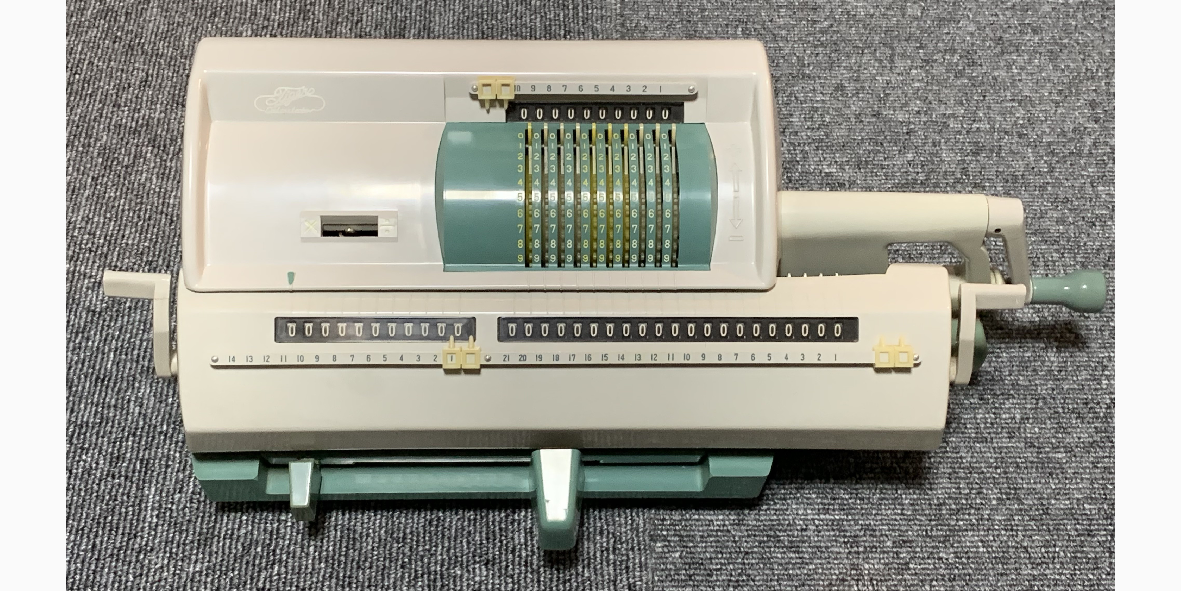
\includegraphics[page=1,width=\linewidth]{./images/pictures.pdf}

  \note{
    ネットワークの代表格であるとろの
    インターネットの基本原理について立ち返るよ。
    TCP/IPでは、より上位から順に、
    アプリケーション層、トランスポート層、インターネット層、リンク層の
    4つの階層から成っているよ。

    アプリケーション層は、例えばWebやVRChatといったサービス、
    名前解決やアドレス自動割り当てなどの機能を実現するよ。
    トランスポート層は、Webのデータをブラウザへ、
    VRChatのデータをVRChatへといった具合に
    適切な通信を適切なアプリケーションに届けるよ。
    インターネット層では、世界中を張り巡らされた数多のネットワークを通り抜け、
    目的のホスト(コンピュータ)までデータを届けるよ。
    リンク層では、そのホストから物理的に直接通信できる範囲でデータを届けるよ。

    これらの層が連携して仕事をすることで様々な通信を実現できるよ。
  }
\end{frame}

\begin{frame}
  \frametitle{情報を伝える根幹のしくみ}

  \includegraphics[page=2,width=\linewidth]{./images/pictures.pdf}

  \note{
    今回のお話では、これらの層の一番下位の部分、リンク層に着目するよ。

    リンク層で用いられるプロトコルとして、
    LANケーブルに電気を通したり、光ファイバに光を通したりして
    通信するEthernetや電波を遣って通信をするWi-Fiなどがあるよ。
    また、少し古めかしいところではダイヤルアップ通信
    (電話線とモデムとを使ったPPP)もリンク層の通信だよ。
    この場合、コンピュータは電話を使って「直接」通信していることになるよ。

    TCP/IPでは下位の層は上位の層にデータを受け渡せれば良いよ。
    つまり、リンク層では、同一リンク内で通信でき、
    適切にデータを伝送できれば良いので、
    ここで用いる伝送方式はかなり自由に選択できるよ。
    「味のあるリンク」で当たり前の通信を実現できると面白そうだね。
  }
\end{frame}

\section{鳥類キャリアによるIP通信}
\note{
  ここで、「味のあるリンク」であるところの
  鳥類キャリアについて思いを馳せていくよ。
}

\begin{frame}
  \frametitle{RFC 1149: 1990年4月1日発のジョークRFC}

  鳥類キャリアを用いたIP通信の手法が検討されている\cite{RFC1149}\\
  \hspace{1.5\zw}QoSの提供\cite{RFC2549}やIPv6への対応\cite{RFC6214}など改良・拡張されている

  2001年 ノルウェーで実装実験が行われた
  \begin{itemize}
    \item
      6羽のハトを使ってpingパケットを伝送
    \item
      道中、別のハトの群れと一緒に寄り道するなど
    \item
      4羽がパケットを持って戻ってきた(33\%の損失)
    \item
      往復通信時間は3211秒から6389秒までさまざま
  \end{itemize}

  \note{
    興味深いリンクの手法として、「鳥類キャリア」があるよ。
    これは、情報を伝える手段として、電気や電波の代わりに
    鳥類(つまり伝書鳩など)を用いるものだよ。
    実験用のプロトコルとしてRFCに規格があるよ。
    当然、ジョークのRFCであるが、QoSの検討やIPv6への対応も図られているよ。

    実装も試みられていて、2001年にはノルウェーで実験が行われているよ。
    この実験では6羽のハトを使ってpingパケットを伝送したよ。
    この日は現地では珍しい晴れの日であったようで、
    道中別のハトの群れと一緒に一時間ほど寄り道するなどしていたようだよ。
    パケットは無事に相手の端へ辿り着き、4羽が応答パケットを持って帰ってきたよ。
    パケロス率は33\%、
    RTTは3211秒から6389秒まで(大体1--2時間程度)であったようだよ。
  }
\end{frame}

\begin{frame}
  \frametitle{鳥類キャリアを用いたIP通信の手順}

  \begin{enumerate}
      \setcounter{enumi}{-1}
    \item
      IPデータグラムが生成される
    \item
      IPデータグラムを小さな細長い紙に16進数で印刷する
    \item
      鳥の脚に紙を巻き付け、テープで止める
    \item
      鳥を目的の端に飛ばす
      \vspace{\zh}
    \item
      飛んできた鳥の脚に巻き付けられた紙切れを剥がす
    \item
      紙に印刷されているデータグラムを読み取る
    \item
      コンピュータはデータグラムを処理する
  \end{enumerate}

  \note{
    鳥類キャリアによるIP通信はスライドに示される手段で行われるよ。

    IPデータグラムはそのまま(ヘッダなどを付けることなく)
    16進数で印刷されるよ。
    ヘッダを付けてしまうと、
    頭を切り落とされたときに伝送パフォーマンスが下がることが懸念されているよ。

    データグラムの読み取りにはOCRを使っても良いし、人間を使っても良いよ。
  }
\end{frame}

\begin{frame}
  \frametitle{鳥類キャリアを用いたIP通信の特徴}

  \vspace{.25\zh}
  \begin{itemize}
    \item
      通信の帯域幅は鳥の脚の長さによる(時間経過で変化)
    \item
      キャリアは喪失し得る(がIPとしては問題ない)
    \item
      MTUは鳥によって可変(典型的には\qty{256}{\milli\gram})
    \item
      用いる鳥の種類によってQoSを設定できる
    \item
      ブロードキャスト・マルチキャストはむつかしい
    \item
      IPv4とIPv6とを区別するにはIPヘッダを見るしかない
    \item
      位置(地域)によってはキャリアのホップが短い
    \item
      盗聴(覗き見)によるセキュリティ上の懸念がある
  \end{itemize}

  \note{
    RFCの本文で述べられている実用的な特徴はスライドに示す通りだよ。
    重要なところを紹介するよ。
    IPはベストエフォートの通信を提供するので、キャリアは喪失しても問題ないよ。
    MTUやQoSについては鳥の運用期間や種類によって設定されるよ。
    これらについては、人間の関与できるところではないので、
    キャリア特有の問題だと考えられるよ。
    また、鳥のヘッダを見てもパケットの種別を判断できないので、
    IPv4とIPv6との区別はこのレイヤで判別できないよ。
    これは、将来的にIPよりも素晴らしいプロトコルが登場したときに不便だよ。
  }
\end{frame}

\section{郵便を用いたIP通信}
\note{
  ということで、鳥類キャリアのかわりに郵便を用いることについて考えてみるよ。
}

\begin{frame}
  \frametitle{郵便を用いたIP通信}

  \vspace{\zh}
  キャリアとして鳥類のかわりに郵便を用いる\\
  \hspace{1.5\zw}→ 鳥類キャリア特有の制約を取り払える

  \includegraphics[page=1,width=\linewidth]{./images/halfpictures.pdf}

  \note{
    この通信方式では
    鳥類キャリアによるIP通信をベースに、
    キャリアとして鳥類の代わりに郵便を用いることで
    鳥類キャリア特有の制約を取り払うよ。

    つまり、鳥によって運ばれていたパケットを郵便によって運ぶほかは
    基本的に鳥類キャリアを用いたIP通信を基にしているよ。
  }
\end{frame}

\begin{frame}
  \frametitle{郵便を用いたIP通信の手順}

  \begin{enumerate}
      \setcounter{enumi}{-1}
    \item
      IPデータグラムが生成される
    \item
      IPデータグラムを便箋などに印刷する
    \item
      便箋を封筒に入れ、必要な金額の切手を貼る
    \item
      ポストに投函する
      \vspace{\zh}
    \item
      家の郵便受けに届いた封筒から便箋を取り出す
    \item
      便箋に印刷されているデータグラムを読み取る
    \item
      コンピュータはデータグラムを処理する
  \end{enumerate}

  \note{
    郵便によるIP通信はスライドに示される手段で行われるよ。

    鳥類キャリアによる通信と比較してみると、
    鳥に関連している部分が郵便に置き換えられているだけだよ。
  }
\end{frame}

\begin{frame}
  \frametitle{鳥類キャリア vs. 郵便}

  \textbf{パケット喪失率を低減できる}\\
  \hspace{1.5\zw}郵便は鳥類よりもリンクの信頼性が高い

  \textbf{QoSを確実にコントロールできる}\\
  \hspace{1.5\zw}速達やレターパックなどさまざまなサービスを選択できる\\
  \hspace{1.5\zw}特定記録や簡易書留などでパケットの到達を保証できる

  \textbf{通信の大容量化を実現できる}\\
  \hspace{1.5\zw}重さによる制限が緩和される(\qty{256}{\milli\gram} → \qty{50}{\gram})\\
  \hspace{1.5\zw}一度に送信可能なデータ量は封筒の大きさで選択できる\\
  \hspace{1.5\zw}16進数だけでなく、Base64やQRコードなどにも対応できる

  \note{
    鳥類キャリアを用いた通信に比べた郵便を用いた通信の特徴を述べてみるよ。

    まず、パケット喪失率を低減できるようになるよ。
    郵便は鳥類キャリアよりもリンクの信頼性が高いからだよ。
    また、QoSを確実にコントロールできるようになるよ。
    速達などのオプションを利用すればパケットを速く届けられるし、
    特定記録などを利用すればパケットの到達を保証できるよ。
    さらに、通信の大容量化を実現できるよ。
    重さによる制限が約200倍改善されるので、
    より多くのデータを一度に送れるようになるよ。
    普通は紙でデータを送ることになると思うけれども、
    紙は鳥の脚に巻き付けられることかた解き放たれているので、
    この大きさは封筒の大きさに合わせて自由に選択できるよ。
    紙面が広がったことで、16進数だけでなく、
    Base64やQRコードを印刷することもできるよ。
  }
\end{frame}

\section{システムの実装}
\note{
  机上の空論ではつまらないので、これらについて実装を行ったよ。
}

\begin{frame}
  \frametitle{前座: 通常の通信のシステム構成}

  \includegraphics[page=3,width=\linewidth]{./images/pictures.pdf}

  \note{
    ここで、通常のデバイスによる通信に思いを馳せてみよう。
    通常、デバイスはカーネルが管理しているよ。
    当然、デバイスはカーネルと直接会話をするよ。
    そのため、より低レイヤ(OSI参照モデルでL2以下、リンク層)の通信は
    通常であればユーザの世界に出てこないよ。
    この方式によって愚直に実装しようと思えば、
    デバイスの開発やカーネルの修正など、膨大な作業が必要になってしまい、
    現実的ではないよ。
  }
\end{frame}

\begin{frame}
  \frametitle{ダイヤルアップ通信に思いを馳せる}

  ダイヤルアップ通信は本質的にPPP\\
  \hspace{1.5\zw}PPPではシリアルデバイスによってネットワーク接続を実現

  シリアルデバイスはユーザの世界に露出している\\
  \hspace{1.5\zw}Unixの世界ではシリアルデバイスをファイルと同様に扱える\\
  \hspace{1.5\zw}pppdのマネをすればユーザの世界から通信を吹き込める

  pppdはTUN/TAPを用いることで仮想的なNICを生やす\\
  \hspace{1.5\zw}同様の手法で「普通のプログラム」でも通信を吹き込める

  \note{
    ここで、ダイヤルアップ通信に思いを馳せてみよう。
    ダイヤルアップ通信というのは本質的にPPPというプロトコルで通信しているよ。
    PPPではシルアルデバイスによってネットワーク接続を実現しているよ。

    ここで、よく考えてみると、シリアルデバイスというものは
    デバイスファイルとしてユーザの世界に露出していて、
    これはファイルのように読み書きできるよ。
    PPPを実現するpppdのマネをすれば
    ユーザの世界から通信を吹き込めるということなので、
    これについて調べてみると、
    TUN/TAP(トンネルデバイス)を利用して仮想的なNICを生成しているようだよ。
    つまり、
    これを利用すると「普通のプログラム」からでも通信を実現できるようだよ。
  }
\end{frame}

\begin{frame}
  \frametitle{LoLLIPoP: Lots of Latency Letter IP over Post}

  \includegraphics[page=4,width=\linewidth]{./images/pictures.pdf}

  \note{
    これを踏まえて郵便によるIP通信システムLoLLIPoPを開発したよ。
    LoLLIPoPでは、TUN/TAPを利用して仮想NICを用意し、
    さらにパケットの入出力のためのインタフェイスを用意するよ。
    システムはdaemonとCLI tool chainとに分かれていて、
    daemonは入出力インタフェイスとNICとの間でデータを取り次ぐよ。
    CLI tool chainはユーザと入出力インタフェースとの間でデータを取り次ぐよ。
    ネットワークを利用して通信するプログラムからは通常のNICと同様に見えるから、
    pingやその他のプログラムをそのまま利用できるよ。

    あと、パケットの先頭に疑似ヘッダを添えることで
    将来登場するより素晴しいプロトコルにも対応できるようにしているよ。
  }
\end{frame}

\section{通信の実験}
\note{
  開発したシステムをつかって、通信実験を行ってみたよ。
}

\begin{frame}
  \frametitle{10月28日: パケットの生成、送信}

  各方面へのpingパケットをQRコードの形式で印刷、送信

  \begin{center}
    \begin{tabular}{cc}
      \includegraphics[width=0.45\linewidth]{./images/IMG_7302.jpeg} &
      \includegraphics[width=0.45\linewidth]{./images/IMG_7303.jpeg} \\
    \end{tabular}
  \end{center}

  \note{
    10月28日、pingパケットが生成され、QRコードの形式で印刷、送信されたよ。
    このとき、パケットの形状としては郵便書簡が用いられたよ。
    郵便書簡ははがきと同額でありながら封筒のように使えるのでお得だよ。
  }
\end{frame}

\begin{frame}
  \frametitle{10月30日: パケットの着信報告}

  各方面からパケットの着信報告が寄せられる

  \centering
  \includegraphics[width=.8\linewidth]{./images/IMG_7354.PNG}

  \note{
    二日経って、パケットの着信報告が各方面から寄せられたよ。
    しかし、その報告は嬉しいものではなかったよ。
  }
\end{frame}

\begin{frame}
  \frametitle{通信失敗の原因: パケット形式の不一致}

  送信側が古いバージョンのプログラムを利用していた\\
  \hspace{1.5\zw}パケットの先頭に疑似ヘッダのついていないものを送信した

  \centering
  \includegraphics[width=.8\linewidth]{./images/IMG_7355.PNG}

  \note{
    アホだね〜
  }
\end{frame}

\begin{frame}
  \frametitle{10月31日: 速達でパケットを再送信}

  定型郵便(110円)に速達(300円)をつけると送料は410円\\
  \hspace{1.5\zw}→ 翌日以降、続々と着信報告があった

  \centering
  \includegraphics[width=.8\linewidth]{./images/IMG_7356.PNG}

  \note{
    原因に気付いてすぐパケットを再生成、再送信したよ。
    速達をつけたことで、翌日以降続々と着信報告があったよ。
    きちんと転送速度を制御できていることを確認できたよ。
  }
\end{frame}

\begin{frame}
  \frametitle{11月4日: 初めての返信パケットを受信}

  \includegraphics[width=\linewidth]{./images/IMG_E7357.jpeg}

  \note{
    しばらく待っていると、
    初めての返信パケットが到着したよ。
    QRコードに印刷されたパケットを読み込み、
    LoLLIPoPシステムに入力したところ、
    きちんと処理されたよ。
    そして……
  }
\end{frame}

\begin{frame}
  \frametitle{ping実行結果}

  \includegraphics[width=\linewidth]{./images/ping.png}

  \note{
    pingコマンドの実行結果はこのようになったよ。
  }
\end{frame}

\begin{frame}
  \centering\large
  time${}={}$411791688 ms
  \note{
    4億
    1179万
    1688ミリ秒
    だよ
  }
\end{frame}

\begin{frame}
  \centering\LARGE
  411\,791\,688 ms\\
  ||\\
  \Huge\bfseries
  4.7661日
  \note{
    これはなんと約4.7日に相当するよ。
    アホだね〜。
  }
\end{frame}

\begin{frame}
  \frametitle{往復通信の実験結果}

  全5件のうち3件が往復通信に成功\\
  \hspace{1.5\zw}残りの2件は返信処理中

  \begin{itemize}
    \item
      \qty{411791688}{\milli\second}(郵便書簡)
    \item
      \qty{581116715}{\milli\second}(宅急便)
    \item
      \qty{668453815}{\milli\second}(はがき)
  \end{itemize}
  平均往復時間: \qty{553787406}{\milli\second}(\textbf{6.4095日})

  \note{
    実験の結果をまとめるとこのようになるよ。
    全5件のうち3件が往復通信に成功したよ。
    残りの2件は現在返信処理中であるというウワサを聞いているよ。

    平均の往復時間は5億5378万7406ミリ秒で、大体6日と半分だよ。
  }
\end{frame}

\begin{frame}
  \frametitle{実際に送信されてきた往復パケット}

  \centering
  \includegraphics[width=.75\linewidth]{./images/IMG_7358.jpeg}
\end{frame}

\section{まとめ・検討事項}
\note{
  まとめるよ〜
}

\begin{frame}
  \frametitle{郵便を用いた超低速IP通信システムの検討}

  鳥類キャリアを用いたIP通信に着想を得て\\
  \hspace{1.5\zw}郵便を用いたIP通信システムを検討した\\
  \hspace{1.5\zw}人間によってよりコントロールしやすい通信を実現

  Linux上で動作する実装を試作した\\
  通信実験ではパケットロス率40\%(現時点; 待てば届きそう)\\
  \hspace{1.5\zw}平均往復時間\qty{553787406}{\milli\second}を記録した

  \note{
    郵便を用いた超低速IP通信システムの検討ということで、
    鳥類キャリアを用いたIP通信に着想を得て、
    郵便を用いたIP通信システムを検討したよ。
    キャリアとして郵便を用いることで、
    鳥類特有の制限を取り払うことができ、
    人間によってよりコントロールしやすい通信を実現できるよ。

    これについて、Linux上で動作するトンネルデバイスを用いた実装を試作したよ。
    通信実験ではパケットロス率(これは待てば届きそうだけど)40\%を記録し、
    平均往復時間は5億5378万7406ミリ秒となったよ。
  }
\end{frame}

\begin{frame}
  \frametitle{今後の検討事項}

  PING以外の通信\\
  \hspace{1.5\zw}TCPの3 way handshakeの実現\\
  \hspace{1.5\zw}Wake on Letterなどのアプリケーション開発

  ブロードキャスト・マルチキャストの問題\\
  \hspace{1.5\zw}回覧板(トークンリング)方式による実装\\
  \hspace{1.5\zw}定期刊行物(第三種郵便)による実装

  その他のリンクによる通信\\
  \hspace{1.5\zw}電子メールによるe-LoLLIPoPの検討(MIME type の策定)
\end{frame}

\begin{frame}
  \frametitle{あなたたちも郵便でIP通信をしなさい}

  \includegraphics[width=\linewidth]{./images/lollipop.png}
\end{frame}

\appendix

\begin{frame}[standout]
  おわりです

  \note{
    おわりだよ〜。
  }
\end{frame}

\begin{frame}
  \frametitle{参考資料}

  \beamertemplatetextbibitems
  \setbeamerfont{bibliography item}{size=\footnotesize}
  \setbeamerfont{bibliography entry}{size=\footnotesize}
  \setbeamerfont{bibliography entry author}{size=\footnotesize}
  \setbeamerfont{bibliography entry title}{size=\footnotesize}
  \setbeamerfont{bibliography entry location}{size=\footnotesize}
  \setbeamerfont{bibliography entry note}{size=\footnotesize}
  \begin{thebibliography}{1}
    \bibitem{RFC1122}
      Braden, R.,
      \newblock
      Requirements for Internet Hosts --- Communication Layers\textmd,
      \newblock
      \href{https://doi.org/10.17487/RFC1122}{RFC 1122}, October 1989.

    \bibitem{RFC1149}
      Waitzman, D.,
      \newblock
      Standard for the transmission of IP datagrams on avian carriers\textmd,
      \newblock
      \href{https://doi.org/10.17487/RFC1149}{RFC 1149}, April 1990.

    \bibitem{RFC2549}
      Waitzman, D.,
      \newblock
      IP over Avian Carriers with Quality of Service\textmd,
      \newblock
      \href{https://doi.org/10.17487/RFC2549}{RFC 2549}, April 1999.

    \bibitem{RFC6214}
      Carpenter B., Hinden  R.,
      \newblock
      Adaptation of RFC 1149 for IPv6\textmd,
      \newblock
      \href{https://doi.org/10.17487/RFC6214}{RFC 6214}, April 2011.
  \end{thebibliography}
\end{frame}

\begin{frame}
  \frametitle{このスライドについて}

  Written in November 2025.

  Permanent ID of this document: \texttt{2976cf5d5f923407}.

  Copyright © 2025 KusaReMKN.

  特記無き場合、プログラムやソースコードは MIT License で、\\
  \hspace{1.5\zw}それ以外のコンテンツは CC-BY 4.0 で利用可能です。\\
  \hspace{1.5\zw}一部の画像には別のライセンスが適用されるかもしれません。
\end{frame}

\end{document}
% ex: se et ts=2 :
